\documentclass[10pt,a4paper,landscape]{article}
\usepackage{multicol}
\usepackage{calc}
\usepackage{ifthen}
\usepackage[landscape]{geometry}
\usepackage{hyperref}

\usepackage[utf8]{inputenc}

% Fuentes (Fira Sans)
\usepackage[T1]{fontenc}
\usepackage[sfdefault,scaled=.85]{FiraSans}
\usepackage{newtxsf}
\usepackage[scaled=.85]{FiraMono}

% TikZ for UML

\usepackage{tikz-uml}

% Listings for code

\usepackage{listings}
\lstset{basicstyle=\ttfamily\footnotesize,breaklines=true}

% Multiple cols/rows

\usepackage{multirow}

% Checkmarks

\usepackage{amssymb}

% To make this come out properly in landscape mode, do one of the following
% 1.
%  pdflatex latexsheet.tex
%
% 2.
%  latex latexsheet.tex
%  dvips -P pdf  -t landscape latexsheet.dvi
%  ps2pdf latexsheet.ps


% If you're reading this, be prepared for confusion.  Making this was
% a learning experience for me, and it shows.  Much of the placement
% was hacked in; if you make it better, let me know...


% 2008-04
% Changed page margin code to use the geometry package. Also added code for
% conditional page margins, depending on paper size. Thanks to Uwe Ziegenhagen
% for the suggestions.

% 2006-08
% Made changes based on suggestions from Gene Cooperman. <gene at ccs.neu.edu>


% To Do:
% \listoffigures \listoftables
% \setcounter{secnumdepth}{0}


% This sets page margins to .5 inch if using letter paper, and to 1cm
% if using A4 paper. (This probably isn't strictly necessary.)
% If using another size paper, use default 1cm margins.
\ifthenelse{\lengthtest { \paperwidth = 11in}}
	{ \geometry{top=.5in,left=.5in,right=.5in,bottom=.5in} }
	{\ifthenelse{ \lengthtest{ \paperwidth = 297mm}}
		{\geometry{top=1cm,left=1cm,right=1cm,bottom=1cm} }
		{\geometry{top=1cm,left=1cm,right=1cm,bottom=1cm} }
	}

% Turn off header and footer
\pagestyle{empty}
 

% Redefine section commands to use less space
\makeatletter
\renewcommand{\section}{\@startsection{section}{1}{0mm}%
                                {-1ex plus -.5ex minus -.2ex}%
                                {0.5ex plus .2ex}%x
                                {\normalfont\large\bfseries}}
\renewcommand{\subsection}{\@startsection{subsection}{2}{0mm}%
                                {-1explus -.5ex minus -.2ex}%
                                {0.5ex plus .2ex}%
                                {\normalfont\normalsize\bfseries}}
\renewcommand{\subsubsection}{\@startsection{subsubsection}{3}{0mm}%
                                {-1ex plus -.5ex minus -.2ex}%
                                {1ex plus .2ex}%
                                {\normalfont\small\bfseries}}
\makeatother

% Define BibTeX command
\def\BibTeX{{\rm B\kern-.05em{\sc i\kern-.025em b}\kern-.08em
    T\kern-.1667em\lower.7ex\hbox{E}\kern-.125emX}}

% Don't print section numbers
\setcounter{secnumdepth}{0}


\setlength{\parindent}{0pt}
\setlength{\parskip}{0pt plus 0.5ex}


% -----------------------------------------------------------------------

\begin{document}

\raggedright
\footnotesize
\begin{multicols}{3}


% multicol parameters
% These lengths are set only within the two main columns
%\setlength{\columnseprule}{0.25pt}
\setlength{\premulticols}{1pt}
\setlength{\postmulticols}{1pt}
\setlength{\multicolsep}{1pt}
\setlength{\columnsep}{2pt}


\tikzumlset{font=\footnotesize}

\begin{center}
     \Large{\textbf{PDOO temas 1 y 2}} \\
\end{center}

\section{Conceptos básicos}

\subsection{Envío de mensajes entre objetos}

Diferentes formas de ligar un mensaje al método que lo resuelve

\begin{tabular}{@{}ll@{}}
Estática    & Ocurre antes de la ejecución, más eficiente \\
Dinámica  & Ocurre durante la ejecución, más flexible, la usan Java y Ruby \\
\end{tabular}

\subsection{Especificadores de acceso}

\subsubsection{Java}

\begin{tabular}{cccc}
\multirow{2}{*}{Visible en} & \multicolumn{2}{c}{Mismo paquete} & Otro paquete
  \\
                            & Clase & Otra & Otra \\
  private & \checkmark & - & - \\
  package & \checkmark & \checkmark & - \\
  protected & \checkmark & \checkmark & - \\
  public & \checkmark & \checkmark & \checkmark \\
\end{tabular}

Se utiliza \textit{protected} por defecto. Hay introspección, ya que se
puede consultar una clase u objeto en ejecución.

\subsubsection{Ruby}

\begin{tabular}{cccc}
Visible en & Desde el propio objeto & Clase & Otra\\
  private & \checkmark & - & - \\
  protected & \checkmark & \checkmark & - \\
  public & \checkmark & \checkmark & \checkmark \\
\end{tabular}

Se utiliza \textit{private} por defecto. Se pueden consultar y modificar las
clases, métodos y variables en ejecución. 

\section{Diagramas UML}

\subsection{Diagramas de clases}

\begin{tikzpicture}[]
  \umlclass{Nombre$^{multiplicidad}$}{
    [visibilidad] nombreAtributo [:tipo[multiplicidad]][=valorInicial] \\
    $\vdots$ \\
  }{
    [visibilidad] nombreMétodo ([lista parámetros])[:tipo retorno] \\
    $\vdots$ \\
  }
\end{tikzpicture}

La multiplicidad de la clase indica el número de instancias que puede tener. La
de un atributo, el número de elementos que tiene. La descripción de la responsabilidad de la clase puede indicarse debajo. La
visibilidad se marca mediante:

\begin{tabular}{@{}ll@{}}
\verb!+!    & Pública \\
\verb!-!  & Privada \\
\verb!~! & Paquete \\
\verb!#!  & Protegida \\
\end{tabular}

Para indicar un atributo o método de clase, lo subrayamos.

\subsection{Herencia y ocultamiento de información}
\label{sub:herencia_y_ocultamiento_de_informaci_n}

\begin{tabular}{ccccc}
    \multirow{3}{*}{ Declarado como} & \multicolumn{2}{c}{Java} & \multicolumn{2}{c}{Ruby}\\
                                     & \multicolumn{2}{c}{Subclase} & \multirow{2}{*}{ \begin{tabular}{c}
                                         Propio obj. \\
                                         en la subcl.
                                     \end{tabular}} & \multirow{2}{*}{ \begin{tabular}{c}
                                    Cualquier obj. \\
                                     en la subcl.
                                 \end{tabular} } \\
                                                                   & M. paq. & D. paq. & & \\
private & - & - & \checkmark & - \\
package & \checkmark & - & - & - \\
protected & \checkmark & \checkmark &  \checkmark &  \checkmark   \\
public & \checkmark & \checkmark & \checkmark &  \checkmark  \\
\end{tabular}

\subsection{Redefinición de métodos en Java}
\label{sub:redefinici_n_de_m_todos_en_java}

Utilizamos \texttt{@Override}. La cabecera del método que se redefine puede cambiar la visibilidad y el tipo de retorno. No se puede redefinir un método marcado como \texttt{final}.

\section{Cosas que recordar}
\label{sec:cosas_que_recordar}

En Java si una variable de clase se redefine en una clase cambiando su valor, solo sus subclases verán el nuevo valor.

En Ruby, \texttt{super} sólo permite llamar al método actual, no a cualquier método de la clase padre.

Las clases abstractas no tienen instancias.

Cuando declaramos la referencia a un objeto, \texttt{MiClase objeto = new MiClase} el tipo de la referencia \texttt{objeto} es \texttt{MiClase} y sus subclases.

El casting no cambia el tipo de un objeto. Simplemente indica al compilador el tipo de objeto que se espera en ese momento.

\section{Clases en Java y Ruby}

\subsubsection{Java}
\lstinputlisting[language=Java]{t12cjava.java}

\subsubsection{Ruby}
\lstinputlisting[language=Ruby]{t12cruby.rb}

\end{multicols}
\end{document}
